
\documentclass[11pt]{article}

\usepackage[printonlyused]{acronym}
\usepackage{amsmath}
\usepackage{amssymb}
\usepackage{capt-of}
\usepackage[T1]{fontenc}
\usepackage[margin=2.5cm]{geometry}
\usepackage{graphicx}
\usepackage{grffile}
\usepackage{hyperref}
\usepackage[utf8]{inputenc}
\usepackage{longtable}
\usepackage{rotating}
\usepackage{soul,color}
\usepackage{textcomp}
\usepackage[normalem]{ulem}
\usepackage{wrapfig}

\acrodef{DASH}{Dynamic Adaptive Streaming over HTTP}
\acrodef{ECDF}{Empirical Cumulative Distribution Function}
\acrodef{JMUW}{Julius-Maximilians-Universit\"at W\"urzburg}
\acrodef{JSON}{Java Script Object Notation}
\acrodef{MBB}{Mobile Broadband}
\acrodef{MONROE}{Measuring Mobile Broadband Networks in Europe}
\acrodef{MOS}{Mean Opinion Score}
\acrodef{MPD}{Media Presentation Description}
\acrodef{QoS}{Quality of Service}
\acrodef{QoE}{Quality of Experience}
\acrodef{SRL}{Simula Research Laboratory}
\acrodef{VoD}{Video on Demand}

\author{Cise Midoglu, Anika Schwind}
\date{\today}
\title{VideoMon Project\\\medskip
\large Internal Summary}
\hypersetup{
 pdfauthor={Cise Midoglu, Anika Schwind},
 pdftitle={Braindump},
 pdfkeywords={},
 pdfsubject={},
 pdfcreator={Emacs 25.1.1 (Org mode 9.0)}, 
 pdflang={English}}
\begin{document}

\maketitle
\tableofcontents
\clearpage


\section{Abstract / Executive Summary}\label{sec:abstract}

\textbf{Keywords:} {\ac{DASH}, \ac{QoE}, \ac{QoS}, video}
\clearpage

\section{Introduction}\label{sec:introduction}

\subsection{Motivation}

\begin{itemize}
\item 
\item
\item
\end{itemize}

\subsection{Interested Parties}

\begin{itemize}
\item Network operators:
\begin{itemize}
\item 
\item
\item
\end{itemize}

\item Service providers:
\begin{itemize}
\item 
\item
\item
\end{itemize}

\item End users:
\begin{itemize}
\item 
\item
\item
\end{itemize}

\item Researchers:
\begin{itemize}
\item 
\item
\item
\end{itemize}


\end{itemize}

\clearpage

\section{Related Work}\label{sec:relatedwork}

\subsection{Taxonomy}

\begin{table}[h!]
\centering
\caption{Taxonomy of related work.}
\begin{tabular}{|c|c|c|c|}
\hline
\textbf{Category} & \textbf{Authors} & \textbf{Work} & \textbf{Notes and References} \\
\hline
Adaptation algorithms & & & \\
\hline
Adaptation algorithms & & & \\
\hline
Adaptation algorithms & & & \\
\hline
Adaptation algorithms & & & \\
\hline
Video \ac{QoE} & & & \\
\hline
Video \ac{QoE} & & & \\
\hline
Video \ac{QoE} & & & \\
\hline
... & & & \\
\hline
\end{tabular}
\label{tab:relatedwork}
\end{table}

\subsection{Adaptation Algorithms}


\subsection{Video \ac{QoE}}

\textbf{Seufert et al.} ... \\%~\cite{Seufert2014}} ...\\

\textbf{Wamser et al.} ... \\%~\cite{Wamser2015}} ...\\

\clearpage

\section{Development History}\label{sec:developmenthistory}

\begin{table}[h!]
\centering
\caption{VideoMon development history.}
\begin{tabular}{|c|c|l|c|}
\hline
\textbf{Date} & \textbf{Party} & \textbf{Action} & \textbf{Notes and References} \\
\hline
2015? & \ac{JMUW} & YoMo App & \\
\hline
2016? & \ac{JMUW} & YoMo MONROE container & \\
\hline
x.2016 & \ac{SRL} & AStream MONROE container &\\
\hline
07.2017 & \ac{JMUW}, \ac{SRL} & Initial measurements with YoMo and AStream & \\  
\hline
08.2017 & \ac{JMUW}, \ac{SRL} & Joint work on VideoMon container started & \\  
\hline
10.2017 & \ac{JMUW}, \ac{SRL} & VideoMon beta version, measurement campaign x &\\
\hline
... & & & \\
\hline
\end{tabular}
\label{tab:developmenthistory}
\end{table}
\clearpage

\section{People}\label{sec:people}

\begin{table}[h!]
\centering
\caption{People involved.}
\begin{tabular}{|c|c|l|c|}
\hline
\textbf{Institution} & \textbf{Person} & \textbf{Contact} & \textbf{Tasks} \\
\hline
\ac{JMUW} & Schwind, Anika & & \\
\hline
\ac{JMUW} & Seufert, Michael? & & \\
\hline
\ac{JMUW} & Wamser, Florian & & \\
\hline
\ac{SRL} & Alay, \"Ozg\"u & \url{https://www.simula.no/people/ozgu} & \\
\hline
\ac{SRL} & Midoglu, Cise & \url{https://www.simula.no/people/cise} & \\
\hline
\end{tabular}
\label{tab:people}
\end{table}


\subsection{\ac{JMUW}}

\subsection{\ac{SRL}}

\textbf{Cise Midoglu} was born in 1989 in Ankara. She studied Electrical and Electronics Engineering at Bilkent University where she received her B.Sc. degree in 2010. She received her M.Sc. degree in Information Technology with a specialization in Communication Engineering and Media Technology from the University of Stuttgart in 2013. She was employed at the Institute of Telecommunications as a project assistant within the Mobile Communications Group between 2015 and 2016. She is working as a PhD Student at Simula Research Laboratory since 2016 under the supervision of \"Ozg\"u Alay.
\clearpage

\section{\ac{MONROE}}\label{sec:monroe}

\clearpage

\section{YoMo}\label{sec:yomo}

\subsection{Container Design}
\clearpage

\section{AStream}\label{sec:astream}

\subsection{Original Implementation}

\subsection{Container Implementation for \ac{MONROE}}
\clearpage

\section{VideoMon}\label{sec:videomon}

\subsection{Container Design}
\clearpage

\section{Measurements}

\subsection{Measurement Setup}

\subsection{Measurement Campaigns}

Table~\ref{tab:measurements} lists the measurement campaigns.

\begin{table}[h!]
\centering
\caption{Measurement campaigns.}
\begin{tabular}{|c|c|c|c|}
\hline
\textbf{Date} & \textbf{Number of Batches} & \textbf{Number of Nodes} & \textbf{Other} \\
\hline
&&&\\
\hline
&&&\\
\hline
&&&\\
\hline
\end{tabular}
\label{tab:measurements}
\end{table}




\clearpage

\section{Analysis}\label{sec:analysis}

Minimal plots using summary \ac{JSON}:
\begin{itemize}
\item Barchart (mean, max, min, q1, q2, q3, q4) of bitrate
\item Barchart (mean, max, min, q1, q2, q3, q4) of buffer
\item Barchart (mean, max, min, q1, q2, q3, q4) of stall duration
\item Barchart of number of switches (up), number of switches (down),  number of stalls
\end{itemize}


Advanced plots:
%\begin{itemize}
%\item  Buffer vs. time, buffer+playback+downloaded playtime vs. time
%\item Bitrate vs. time
%\item \ac{ECDF} of bitrate OR (barchart?) percentile-min-max-mean comparison
%\item YouTube vs. AStream of bitrate
%\item Time spent on each quality level YouTube vs. AStream
%\item (barchart?) num. Switches, num. Stalls YouTube vs. AStream
%\end{itemize}

\begin{itemize}
\item Bitrate
\begin{itemize}
\item Bitrate (Kbps) vs. Time (s), YoMo and AStream
\item \ac{ECDF} of bitrate (Kbps), YoMo and AStream
\end{itemize}
\item Buffer
\begin{itemize}
\item Buffer (s) vs. Time (s), YoMo and AStream 
\item Buffer (s) + playback (s) + downloaded playtime (s) vs. Time (s), YoMo
\item Buffer (s) + playback (s) + downloaded playtime (s) vs. Time (s), AStream
\end{itemize}
\item Quality levels
\begin{itemize}
\item Time spent at each (s) vs. Level (name), barchart, YoMo and AStream
\item Switch and Stalls
\item Num. up switches, num. Down switches, num. Stalls, YoMo and AStream
\end{itemize}
\end{itemize}

\begin{figure} [h!]
\caption{Sample plots.}
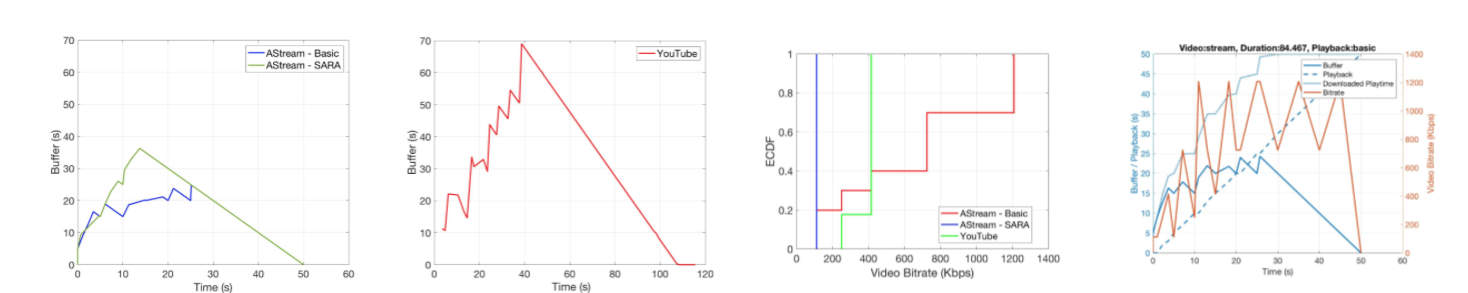
\includegraphics[width=\textwidth]{graphics/sampleplots}
\label{fig:sampleplots}
\end{figure}

\begin{figure} [h!]
\caption{Flo notes.}
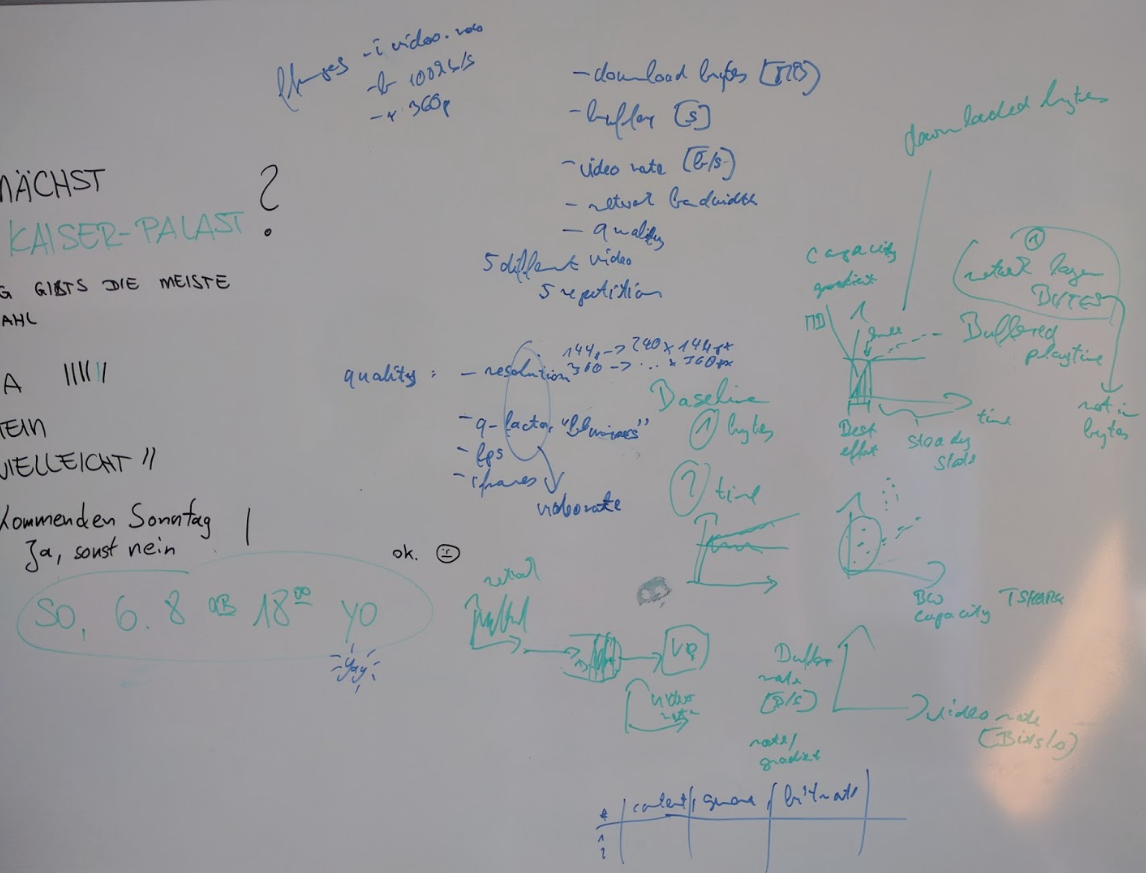
\includegraphics[width=\textwidth]{graphics/flonotes}
\label{fig:flo notes}
\end{figure}

\clearpage

\section{Discussion}\label{sec:discussion}

\subsection{Adaptation Algorithms}

\subsection{Video Content}

\subsection{Network Operators}

\subsection{Location}

\subsection{Time of Day}

\subsection{End Devices}

\subsection{Mobility}
\clearpage

\section{Conclusion}\label{sec:conclusion}




\bibliographystyle{IEEEtran}
\bibliography{references}

\end{document}